\documentclass[a4paper]{article}

\usepackage[utf8]{inputenc}
\usepackage[T2A]{fontenc}
\usepackage[russian]{babel}

\usepackage{mathtext}

\usepackage{listings}
\usepackage{color}

\definecolor{mygreen}{rgb}{0,0.6,0}
\definecolor{mygray}{rgb}{0.5,0.5,0.5}
\definecolor{mymauve}{rgb}{0.58,0,0.82}

\lstset{
	morekeywords={*,...}, % если хотите добавить ключевые слова
	keywordstyle=\color{blue},
	stringstyle=\color{mymauve},
	% Настройки отображения
	breaklines=true, % Перенос длинных строк
	basicstyle=\footnotesize, % Шрифт для отображения кода
	backgroundcolor=\color{white}, % Цвет фона кода
	frame=single,
	rulecolor=\color{black}, % Цвет рамки
	tabsize=3, % Размер табуляции в пробелах
	% Настройка отображения номеров строк. Если не нужно, то удалите весь блок
	numbers=left, % Слева отображаются номера строк
	stepnumber=1, % Каждую строку нумеровать
	numbersep=5pt, % Отступ от кода
	numberstyle=\tiny\color{mygray},
	% Для отображения русского языка
	extendedchars=true,
	literate={Ö}{{\"O}}1
	{Ä}{{\"A}}1
	{Ü}{{\"U}}1
	{ß}{{\ss}}1
	{ü}{{\"u}}1
	{ä}{{\"a}}1
	{ö}{{\"o}}1
	{~}{{\textasciitilde}}1
	{а}{{\selectfont\char224}}1
	{б}{{\selectfont\char225}}1
	{в}{{\selectfont\char226}}1
	{г}{{\selectfont\char227}}1
	{д}{{\selectfont\char228}}1
	{е}{{\selectfont\char229}}1
	{ё}{{\"e}}1
	{ж}{{\selectfont\char230}}1
	{з}{{\selectfont\char231}}1
	{и}{{\selectfont\char232}}1
	{й}{{\selectfont\char233}}1
	{к}{{\selectfont\char234}}1
	{л}{{\selectfont\char235}}1
	{м}{{\selectfont\char236}}1
	{н}{{\selectfont\char237}}1
	{о}{{\selectfont\char238}}1
	{п}{{\selectfont\char239}}1
	{р}{{\selectfont\char240}}1
	{с}{{\selectfont\char241}}1
	{т}{{\selectfont\char242}}1
	{у}{{\selectfont\char243}}1
	{ф}{{\selectfont\char244}}1
	{х}{{\selectfont\char245}}1
	{ц}{{\selectfont\char246}}1
	{ч}{{\selectfont\char247}}1
	{ш}{{\selectfont\char248}}1
	{щ}{{\selectfont\char249}}1
	{ъ}{{\selectfont\char250}}1
	{ы}{{\selectfont\char251}}1
	{ь}{{\selectfont\char252}}1
	{э}{{\selectfont\char253}}1
	{ю}{{\selectfont\char254}}1
	{я}{{\selectfont\char255}}1
	{А}{{\selectfont\char192}}1
	{Б}{{\selectfont\char193}}1
	{В}{{\selectfont\char194}}1
	{Г}{{\selectfont\char195}}1
	{Д}{{\selectfont\char196}}1
	{Е}{{\selectfont\char197}}1
	{Ё}{{\"E}}1
	{Ж}{{\selectfont\char198}}1
	{З}{{\selectfont\char199}}1
	{И}{{\selectfont\char200}}1
	{Й}{{\selectfont\char201}}1
	{К}{{\selectfont\char202}}1
	{Л}{{\selectfont\char203}}1
	{М}{{\selectfont\char204}}1
	{Н}{{\selectfont\char205}}1
	{О}{{\selectfont\char206}}1
	{П}{{\selectfont\char207}}1
	{Р}{{\selectfont\char208}}1
	{С}{{\selectfont\char209}}1
	{Т}{{\selectfont\char210}}1
	{У}{{\selectfont\char211}}1
	{Ф}{{\selectfont\char212}}1
	{Х}{{\selectfont\char213}}1
	{Ц}{{\selectfont\char214}}1
	{Ч}{{\selectfont\char215}}1
	{Ш}{{\selectfont\char216}}1
	{Щ}{{\selectfont\char217}}1
	{Ъ}{{\selectfont\char218}}1
	{Ы}{{\selectfont\char219}}1
	{Ь}{{\selectfont\char220}}1
	{Э}{{\selectfont\char221}}1
	{Ю}{{\selectfont\char222}}1
	{Я}{{\selectfont\char223}}1
	{і}{{\selectfont\char105}}1
	{ї}{{\selectfont\char168}}1
	{є}{{\selectfont\char185}}1
	{ґ}{{\selectfont\char160}}1
	{І}{{\selectfont\char73}}1
	{Ї}{{\selectfont\char136}}1
	{Є}{{\selectfont\char153}}1
	{Ґ}{{\selectfont\char128}}1
	{\{}{{{\color{black}\{}}}1 % Цвет скобок {
	{\}}{{{\color{black}\}}}}1 % Цвет скобок }
	,
%	title=\lstname
}

\usepackage{algorithmicx}
\usepackage{algpseudocode}

\usepackage{amssymb}
\usepackage{amsopn}
\usepackage{mathtools}

\usepackage{graphicx}

\usepackage[
a4paper, includefoot,
left=2cm, right=1cm, top=2cm, bottom=2cm,
]{geometry}

\usepackage[hidelinks]{hyperref}
\usepackage{multirow}
\usepackage{cmap}


\begin{document}

\begin{titlepage}

	\begin{center}

		\large Федеральное государственное автономное образовательное учреждение высшего образования \\
		\large «Санкт-Петербургский политехнический университет Петра Великого» \\
		\large Институт компьютерных наук и технологий \\
		\large Кафедра «Компьютерные интеллектуальные технологии» \\[4cm]

		\huge {\bf Курсовая работа} \\[0.5cm]
		\large {\bf Информационная система автомобилестроительного предприятия} \\[0.1cm]
		\large по дисциплине «Базы данных» \\[4cm]

	\end{center}

    \begin{center}
        \begin{minipage}[t]{4cm}
            \begin{flushleft}
                Выполнил студент гр. 23506/1
            \end{flushleft}
        \end{minipage}
        \hfill
        \begin{minipage}[t]{4cm}
            \begin{flushright}
            О.Д. Романов
            \end{flushright}
        \end{minipage} \\[0.5cm]

        \begin{minipage}[t]{4cm}
            \begin{flushleft}
                Руководитель старший преподаватель
            \end{flushleft}
            \flushleft
        \end{minipage}
        \hfill
        \begin{minipage}[t]{4cm}
            \begin{flushright}
                Н.В. Андреева
            \end{flushright}
        \end{minipage}
    \end{center}

    \begin{flushright}
        14 мая 2017
    \end{flushright}

	
	\vfill

	\begin{center}
	    \large Санкт-Петербург\\
	    \large \the\year
	\end{center}
 
\end{titlepage}

\section*{Задание на проектирование}

{\bf Срок сдачи законченной работы: } 22.05.2017

\underline{Начальное описание предметной области:}

Структурно предприятие состоит из цехов, которые в свою очередь подразделяются на участки.

Категории изделий, выпускаемых предприятием: грузовые, легковые автомобили, автобусы, сельскохозяйственные, дорожно-строительные машины, мотоциклы и прочие изделия.
Каждая категория изделий имеет специфические, присущие только ей атрибуты.
Например, для автобусов это вместимость, для сельскохозяйственных и дорожно-строительных машин - производительность и т.д.

По каждой категории изделий может собираться несколько видов изделий (под видом изделия понимается конкретная его разновидность / марка - например, автомобиль KIA Rio).
По конкретным экземплярам каждого вида ведётся журнал, где отмечаются даты завершения различных этапов жизненного цикла изделия: изготовление (сборка) / тестирование / передача дилеру / гарантийный ремонт.

Предприятие в основном состоит из производственных цехов, но также есть несколько вспомогательных (например, ремонтный, тестировочный).

Каждая категория изделий собирается в своём производственном цехе (в одном цехе может собираться несколько категорий изделий).
Цех структурно состоит из участков, на каждом из которых выполняется один вид работ: изготавливается определённая часть изделия (например, двигатель) либо производится сборка изделия в целом.
С каждой категорией изделия ассоциируется свой набор работ; другими словами, каждая категория в процессе изготовления должна пройти определённый набор участков в цехе.

Каждой категории инженерно-технического персонала (инженеры, технологи, техники) и рабочих (сборщики, токари, слесари, сварщики и пр.) также характерны атрибуты, свойственные только для этой группы.
Рабочие объединяются в бригады, которыми руководят бригадиры.
Бригадиры выбираются из числа рабочих.
Работу цеха возглавляет начальник цеха, а работу на участке - начальник участка, в подчинении которого находится несколько мастеров.
Каждый мастер координирует работу одной или нескольких бригад (но, в отличие от бригадира, не входит в состав конкретной бригады).
Мастера, начальники участков и цехов назначаются из числа инженерно-технического персонала.
Каждый начальник может руководить только одной структурной единицей (в т.ч. начальник одной структурной единицы не может быть в то же время начальником другой).

Работу по сборке конкретной категории изделия на определенном участке выполняет одна бригада рабочих, при этом она может обслуживать несколько участков / категорий и на одном участке может работать несколько бригад.

\begin{enumerate}

    \item Сотрудники могут быть либо из инженерно-технического персонала (ИТП), либо из числа рабочих.
    \item Каждой категории инженерно-технического персонала (инженеры, технологи, техники) и рабочих (сборщики, токари, слесари, сварщики) характерны атрибуты, свойственные только для этой группы.
    \item Рабочие объединяются в бригады
    \item Бригадиры руководят бригадами и выбираются из числа рабочих.
    \item Мастера, начальники участков и цехов назначаются из числа инженерно-технического персонала.
    \item Каждый начальник может руководить только одной структурной единицей (в т.ч. начальник одной структурной единицы не может быть в то же время начальником другой).

\end{enumerate}

\underline{Варианты запросов к информационной системе:}
\begin{enumerate}

    \item Перечень видов изделий по категории, собираемой указанным цехом.
    В последней строке вывести общее число собираемых видов изделий.

    \item Количество экземпляров изделий каждого вида каждой категории, собранных предприятием за определенный отрезок времени.
    В последней строке вывести общее число собранных изделий.
    Примерный вид результата:

    \begin{tabular}{|p{6cm}|p{2cm}|p{1cm}|} \hline
        Категория & Вид & Кол-во \\ \hline
        Автобусы & АКБ-12 & 8 \\ \hline
        Автобусы & АКБ-05 & 0 \\ \hline
        Автомобили & ИЖ-400 & 12 \\ \hline
        ... & ... & ... \\ \hline
        Всего собрано (12.05.2010-18.07.2010): & & 48 \\ \hline
    \end{tabular}

    \item Данные о кадровом составе (ФИО, должность) по указанным категориям инженерно-технического персонала и рабочих;
    \item Число и перечень участков предприятия и их начальников (с указанием цехов).
    \item Перечень работ, которые проходит указанный вид изделия.
    \item Состав бригад, работающих на указанном участке указанного цеха: ФИО рабочего, номер бригады, номер участка, номер цеха. Отсортировать по номеру бригады.
    \item Перечень мастеров (ФИО) указанного участка указанного цеха и номера бригад, работы которых они координируют.
    \item Информация о цехах, в которых в настоящий момент собирается больше видов изделий, чем в среднем приходится на каждый производственный цех предприятия: номер цеха, название цеха, кол-во собираемых видов изделий, среднее количество видов изделий по цехам предприятия.
    \item Состав бригад, участвующих в сборке указанной категории изделия.
    \item ФИО и должности работников цеха, в котором собирается больше всего категорий изделий.

\end{enumerate}

{\bf Перечень подлежащих разработке вопросов:}
\begin{enumerate}
    \item Проанализировать предметную область, описание которой приведено в выданном варианте задания, и создать логическую модель базы данных.
    \item Провести нормализацию разработанной модели до 5НФ.
    \item Проверить разработанную модель средствами Data Model Validator.
    \item Устранить все замечания по модели, которые выявил Data Model Validator.
    \item Создать физическую модель базы данных, предусмотрев значения по умолчанию и условия проверки вводимых пользователем значений.
    \item Провести прямое проектирование – создать объекты базы данных в Oracle.
    \item Провести обратное проектирование базы данных из Oracle. Убедиться в том, что полученные в результате модели полностью аналогичны исходным.
    \item Проверить корректность произведённого прямого проектирования и выполнение требований, приведённых в описании предметной области (наличие ключей, значений по умолчанию, условий проверки вводимых пользователем значений, связей между таблицами и др.). Проверку произвести, внеся в таблицы базы данных минимум по 5 записей.
    \item Создать 10 SQL-запросов согласно выданному варианту задания. Проверить работоспособность написанных запросов.
    \item Добавить в физическую модель представление на основе SQL-запроса, выбранного по согласованию с преподавателем.
    \item Провести прямое проектирование (перенести созданное представление). Проверить работоспособность представления.
\end{enumerate}

\newpage
\tableofcontents
\newpage

\section{Введение}
В современном мире человек буквально на каждом шагу сталкивается с различными информационными системами.
Начиная от базы данных маленькой школы и заканчивая большими дата-центрами больших компаний.
Однако чем больше необходимо хранить информации, тем больше ее необходимо грамотно (нормализованно) хранить.
Система управления базами данных (СУБД) позволяет создать базу данных, хранить и обновлять в ней данные, а также
СУБД Oracle может быть использована в такой области деятельности, как автомобилестроительное предприятие.
Что я и покажу в данной курсовой работе.

Целью данной работы является спроектировать информационную систему автомобилестроительного предприятия, учитывая техническое задание.

Задачи, которые необходимо выполнить для достижения поставленной цели, перечислены в задании на проектирование.

\newpage

\section{Описание логической модели базы данных}

Диаграммы логической и физической моделей базы данных приведены в Приложении 1 и Приложении 2 соответственно.

\subsection{Сущности, их харрактеристики и связи}
В ходе анализа начального описания предметной области были выявлены следующие сущности:

\begin{enumerate}
    \item{Сотрудник}

    \begin{tabular}{|p{7cm}|p{3cm}|p{1cm}|p{1cm}|p{3cm}|} \hline

        {\bf COLUMN\_NAME} & {\bf DATA\_TYPE} & {\bf PK} & {\bf FK} & {\bf NULLABLE} \\ \hline
        Номер\_договора & VARCHAR2(6) & YES & NO & NO \\ \hline
        Имя\_сотрудника & VARCHAR2(14) & NO & NO & NO \\ \hline
        Фамилия\_сотрудника & VARCHAR2(16) & NO & NO & NO \\ \hline
        Отчество\_сотрудника & VARCHAR2(16) & NO & NO & YES \\ \hline
        Тип\_сотрудника & VARCHAR2(1) & NO & NO & NO \\ \hline
        Дата\_рождения & DATE & NO & NO & YES \\ \hline
        Код\_сотрудника & VARCHAR2(15) & NO & NO & NO \\ \hline
        Должность\_сотрудника & VARCHAR2(8) & NO & NO & NO \\ \hline

    \end{tabular}

    На предприятии работают \underline{сотрудики} (в них входят рабочие и представители инженерно-технического персонала) (1).

    \begin{tabular}{|p{7cm}|p{9.3cm}|} \hline

        {\bf COLUMN\_NAME} & {\bf Примечание} \\ \hline
        Номер\_договора &  Договор о найме на роботу, уникален для каждого сотрудника \\ \hline
        Имя\_сотрудника &  Имя сотрудника, не уникально \\ \hline
        Фамилия\_сотрудника & Фамилия сотрудника, не уникально \\ \hline
        Отчество\_сотрудника & Отчество сотрудника, у человека может не быть фамилии \\ \hline
        Тип\_сотрудника & Сотрудник может быть либо рабочим, либо представителем ИТП. Является дискриминатором в категориальной связи \\ \hline
        Дата\_рождения & Дата рождения сотрудника может быть не указана \\ \hline
        Код\_сотрудника & Атрибут, созданный для категориальной связи. Состоит из: Тип\_сотрудника, Должность\_сотрудника и Номер\_договора \\ \hline
        Должность\_сотрудника & Должность, которую занимает сотрудник (все должности, которые есть на предприятии) \\ \hline

    \end{tabular}

    Ключевая группа XAK1Сотрудник:

    \begin{tabular}{|p{7cm}|p{9.3cm}|} \hline

        {\bf Имя атрибута} & {\bf Примечание} \\ \hline
        Код\_сотрудника & Альтернативный ключ для категориальной связи \\ \hline

    \end{tabular}

    \underline{Сотрудник} может быть или из \underline{инженерно-технического персонала}, или из числа \underline{рабочих} (1), что и реализовано с помощью категориальной связи между соответствующими сущностями.

    \item{ИТП}

    \begin{tabular}{|p{7cm}|p{3cm}|p{1cm}|p{1cm}|p{3cm}|} \hline

        {\bf COLUMN\_NAME} & {\bf DATA\_TYPE} & {\bf PK} & {\bf FK} & {\bf NULLABLE} \\ \hline
        Код\_сотрудника & VARCHAR2(15) & YES & YES & NO \\ \hline

    \end{tabular}

    \underline{Представитель инженерно-технического персонала} входит в какую-то категорию (\underline{инженер}, \underline{технолог} и \underline{техник}), что реализовано с помощью категориальной связи между соответствующими сущностями.

    \underline{Руководитель} (участок, цех, мастер) выбирается из \underline{ИТП} (5), реализовано с помощью связи один-к-одному между соответствующими сущностями.

    \item{Технолог}

    \begin{tabular}{|p{7cm}|p{3cm}|p{1cm}|p{1cm}|p{3cm}|} \hline

        {\bf COLUMN\_NAME} & {\bf DATA\_TYPE} & {\bf PK} & {\bf FK} & {\bf NULLABLE} \\ \hline
        Код\_сотрудника & VARCHAR2(15) & YES & YES & NO \\ \hline
        Специализация\_технолога & VARCHAR2(12) & NO & NO & NO \\ \hline

    \end{tabular}

    Специализация\_технолога может принимать значения: исследования и практика (2).
    Хранит информацию о специализации технолога: практик он или же исследователь.

    \item{Техник}

    \begin{tabular}{|p{7cm}|p{3cm}|p{1cm}|p{1cm}|p{3cm}|} \hline

        {\bf COLUMN\_NAME} & {\bf DATA\_TYPE} & {\bf PK} & {\bf FK} & {\bf NULLABLE} \\ \hline
        Код\_сотрудника & VARCHAR2(15) & YES & YES & NO \\ \hline
        Специализация\_техника & VARCHAR2(7) & NO & NO & NO \\ \hline

    \end{tabular}

    Специализация\_техника может принимать значения: схемы и чертежи (2).
    Хранит информацию о специализации техника: специалист в области схем или же чертежей.

    \item{Инженер}

    \begin{tabular}{|p{7cm}|p{3cm}|p{1cm}|p{1cm}|p{3cm}|} \hline

        {\bf COLUMN\_NAME} & {\bf DATA\_TYPE} & {\bf PK} & {\bf FK} & {\bf NULLABLE} \\ \hline
        Код\_сотрудника & VARCHAR2(15) & YES & YES & NO \\ \hline
        Специализация\_инженера & VARCHAR2(16) & NO & NO & NO \\ \hline

    \end{tabular}

    Специализация\_инженера может принимать значения: проектирование и прототипирование (2).
    Хранит информацию о специализации инженера: специалист в проектировании или же в прототипировании.

    \item{Рабочий}

    \begin{tabular}{|p{7cm}|p{3cm}|p{1cm}|p{1cm}|p{3cm}|} \hline

        {\bf COLUMN\_NAME} & {\bf DATA\_TYPE} & {\bf PK} & {\bf FK} & {\bf NULLABLE} \\ \hline
        Код\_сотрудника & VARCHAR2(15) & YES & YES & NO \\ \hline
        Номер\_бригады & NUMBER(3, 0) & NO & YES & YES \\ \hline

    \end{tabular}

    \underline{Рабочий} входит в какую-то категорию (\underline{сборщик}, \underline{токарь}, \underline{слесарь} и \underline{сварщик}), что реализовано с помощью категориальной связи между соответствующими сущностями.
    \underline{Рабочий} состоит в \underline{бригаде} (3), что и реализовани с помощью связи один-к-одному между соответствующими сущностями.

    Ключевая группа XIE1Рабочий:

    \begin{tabular}{|p{7cm}|p{9.3cm}|} \hline

        {\bf Имя атрибута} & {\bf Примечание} \\ \hline
        Номер\_бригады & Индекс для FK \\ \hline

    \end{tabular}

    \item{Сборщик}

    \begin{tabular}{|p{7cm}|p{3cm}|p{1cm}|p{1cm}|p{3cm}|} \hline

        {\bf COLUMN\_NAME} & {\bf DATA\_TYPE} & {\bf PK} & {\bf FK} & {\bf NULLABLE} \\ \hline
        Код\_сотрудника & VARCHAR2(15) & YES & YES & NO \\ \hline
        Специализация\_сборщика & VARCHAR2(9) & NO & NO & NO \\ \hline

    \end{tabular}

    Специализация\_сборщика может принимать значения: двигатель, подвеска и кузов (2).
    Хранит информацию о специализации сборщик: в сборке какой части он специализируется.

    \item{Токарь}

    \begin{tabular}{|p{7cm}|p{3cm}|p{1cm}|p{1cm}|p{3cm}|} \hline

        {\bf COLUMN\_NAME} & {\bf DATA\_TYPE} & {\bf PK} & {\bf FK} & {\bf NULLABLE} \\ \hline
        Код\_сотрудника & VARCHAR2(15) & YES & YES & NO \\ \hline
        Разряд\_токаря & NUMBER(1, 0) & NO & NO & NO \\ \hline

    \end{tabular}

    Разряд\_токаря может принимать целые значения от 1 до 7 (2).
    Хранит информацию о разряде токаря: их бывает семь.

    \item{Слесарь}

    \begin{tabular}{|p{7cm}|p{3cm}|p{1cm}|p{1cm}|p{3cm}|} \hline

        {\bf COLUMN\_NAME} & {\bf DATA\_TYPE} & {\bf PK} & {\bf FK} & {\bf NULLABLE} \\ \hline
        Код\_сотрудника & VARCHAR2(15) & YES & YES & NO \\ \hline
        Разряд\_слесаря & NUMBER(1, 0) & NO & NO & NO \\ \hline

    \end{tabular}

    Разряд\_слесаря может принимать целые значения от 1 до 6 (2).
    Хранит информацию о разряде слесаря: их бывает шесть.

    \item{Сварщик}

    \begin{tabular}{|p{7cm}|p{3cm}|p{1cm}|p{1cm}|p{3cm}|} \hline

        {\bf COLUMN\_NAME} & {\bf DATA\_TYPE} & {\bf PK} & {\bf FK} & {\bf NULLABLE} \\ \hline
        Код\_сотрудника & VARCHAR2(15) & YES & YES & NO \\ \hline
        Специализация\_сварщика & VARCHAR2(8) & NO & NO & NO \\ \hline

    \end{tabular}

    Специализация\_сварщика может принимать значения: подвеска и рама (2).
    Хранит информацию о специализации сварщика: специалист в сварке подвески или же рамы.

    \item{Руководитель}

    \begin{tabular}{|p{7cm}|p{3cm}|p{1cm}|p{1cm}|p{3cm}|} \hline

        {\bf COLUMN\_NAME} & {\bf DATA\_TYPE} & {\bf PK} & {\bf FK} & {\bf NULLABLE} \\ \hline
        Код\_сотрудника & VARCHAR2(15) & YES & YES & NO \\ \hline
        Ответственность & VARCHAR2(7) & NO & NO & NO \\ \hline
        Код\_ответств & VARCHAR2(22) & NO & NO & NO \\ \hline

    \end{tabular}

    Была создана как таблица посредник для того, чтобы избежать ошибку Table With Too Many Relationships.

    \begin{tabular}{|p{7cm}|p{9.3cm}|} \hline

        {\bf COLUMN\_NAME} & {\bf Примечание} \\ \hline
        Ответственность & То, чем руководит руководитель: участок, мастер или же цех  \\ \hline
        Код\_ответств & Альтернативный ключ, который используется для связи с цехом, участком и бригадой. Так нельзя будет добавить представителя ИТП сразу начальником и цеха, и участка (6). Состоит из: Ответственность и Код\_сотрудника \\ \hline
    \end{tabular}

    Связана с \underline{Бригада} связью один-ко-многим, так как каждый мастер иожет координировать работу нескольких бригад.
    Связана с \underline{Цех} и \underline{Участок} связью один-к-одному.

    Ключевая группа XAK1Руководитель:

    \begin{tabular}{|p{7cm}|p{9.3cm}|} \hline

        {\bf Имя атрибута} & {\bf Примечание} \\ \hline
        Код\_ответств & Альтернативный ключ для связей, так можно будет проверять соответствие руководителей с их должностями на предпритии \\ \hline

    \end{tabular}

    \item{Бригада}

    \begin{tabular}{|p{7cm}|p{3cm}|p{1cm}|p{1cm}|p{3cm}|} \hline

        {\bf COLUMN\_NAME} & {\bf DATA\_TYPE} & {\bf PK} & {\bf FK} & {\bf NULLABLE} \\ \hline
        Номер\_бригады & NUMBER(3, 0) & YES & NO & NO \\ \hline
        Название\_бригады & VARCHAR2(14) & NO & NO & NO \\ \hline
        Бригадир & VARCHAR2(15) & NO & YES & NO \\ \hline
        Мастер & VARCHAR2(22) & NO & YES & NO \\ \hline

    \end{tabular}

    Ключевая группа XAK1Бригада:

    \begin{tabular}{|p{7cm}|p{9.3cm}|} \hline

        {\bf Имя атрибута} & {\bf Примечание} \\ \hline
        Бригадир & У бригады может быть один бригадир\\ \hline

    \end{tabular}

    Ключевая группа XAK2Бригада:

    \begin{tabular}{|p{7cm}|p{9.3cm}|} \hline

        {\bf Имя атрибута} & {\bf Примечание} \\ \hline
        Название\_бригады & В пределах предприятия название уникально \\ \hline

    \end{tabular}

    Ключевая группа XIE1Бригада:

    \begin{tabular}{|p{7cm}|p{9.3cm}|} \hline

        {\bf Имя атрибута} & {\bf Примечание} \\ \hline
        Мастер & Индекс для FK \\ \hline

    \end{tabular}

    \item{Цех}

    \begin{tabular}{|p{7cm}|p{3cm}|p{1cm}|p{1cm}|p{3cm}|} \hline

        {\bf COLUMN\_NAME} & {\bf DATA\_TYPE} & {\bf PK} & {\bf FK} & {\bf NULLABLE} \\ \hline
        Номер\_цеха & VARCHAR2(4) & YES & NO & NO \\ \hline
        Начальник\_цеха & VARCHAR2(22) & NO & YES & NO \\ \hline
        Название\_цеха & VARCHAR2(14) & NO & NO & NO \\ \hline

    \end{tabular}

    Цех может быть либо производственным, либо вспомогательным, что и реализовано с помощью категориальной связи между соответствующими сущностями.
    Цех структурно состоит из участков.
    Для того, чтобы нельзя было записать цех и в вспомогательный, и в производственный, в каждом подтипе есть проверка, что номер цеха имеет префикс (П и В соответсвенно).
    А сам номер проверяется на соответствие этим префиксам (детальнее в условиях проверки).

    Ключевая группа XAK2Цех:

    \begin{tabular}{|p{7cm}|p{9.3cm}|} \hline

        {\bf Имя атрибута} & {\bf Примечание} \\ \hline
        Начальник\_цеха & Начальник может быть только один \\ \hline

    \end{tabular}

    Ключевая группа XAK3Цех:

    \begin{tabular}{|p{7cm}|p{9.3cm}|} \hline

        {\bf Имя атрибута} & {\bf Примечание} \\ \hline
        Название\_цеха & Название уникально в пределах предприятия \\ \hline

    \end{tabular}

    \item{Вспомогательный\_цех}

    \begin{tabular}{|p{7cm}|p{3cm}|p{1cm}|p{1cm}|p{3cm}|} \hline

        {\bf COLUMN\_NAME} & {\bf DATA\_TYPE} & {\bf PK} & {\bf FK} & {\bf NULLABLE} \\ \hline
        Номер\_цеха & VARCHAR2(4) & YES & YES & NO \\ \hline
        Тип\_вспомогательного\_цеха & VARCHAR2(13) & NO & NO & NO \\ \hline

    \end{tabular}

    Номер\_цеха должен иметь перфикс, соответствующий вспомогательному цеху.
    Тип\_вспомогательного\_цеха содержит информацию о типе вспомогательного цеха.
    Например, ремонтный и тестировочный.

    \item{Производственный\_цех}

    \begin{tabular}{|p{7cm}|p{3cm}|p{1cm}|p{1cm}|p{3cm}|} \hline

        {\bf COLUMN\_NAME} & {\bf DATA\_TYPE} & {\bf PK} & {\bf FK} & {\bf NULLABLE} \\ \hline
        Номер\_цеха & VARCHAR2(4) & YES & YES & NO \\ \hline
        Колво\_сбор\_конв & NUMBER(2, 0) & NO & NO & NO \\ \hline

    \end{tabular}

    Номер\_цеха должен иметь перфикс, соответствующий производственному цеху.
    Колво\_сбор\_конв содержит положительное число, которое соответсвует количеству сборочных конвейеров на конкретном производственном цеху.

    \item{Участок}

    \begin{tabular}{|p{7cm}|p{3cm}|p{1cm}|p{1cm}|p{3cm}|} \hline

        {\bf COLUMN\_NAME} & {\bf DATA\_TYPE} & {\bf PK} & {\bf FK} & {\bf NULLABLE} \\ \hline
        Номер\_цеха & VARCHAR2(4) & YES & YES & NO \\ \hline
        Номер\_участка & NUMBER(3, 0) & YES & NO & NO \\ \hline
        Начальник\_участка & VARCHAR2(22) & NO & YES & NO \\ \hline
        Тип\_участка & VARCHAR2(9) & NO & NO & NO \\ \hline
        Название\_участка & VARCHAR2(13) & NO & NO & NO \\ \hline
        Код\_участка & VARCHAR2(16) & NO & NO & NO \\ \hline

    \end{tabular}

    В одном \underline{цеху} может быть несколько \underline{участков}, что и реализовано с помощью связи один-ко-многим между соответствующими сущностями.
    У \underline{участка} может быть один \underline{начальник (руководитель)}, что и реализовано с помощью связи один-к-одному между соответствующими сущностями.
    На участке выполняется один вид работ: изготавливается определённая часть изделия (например, двигатель) либо производится сборка изделия в целом.
    Поэтому \underline{Участок} соединен категориальной связью с \underline{Изготовительный\_участок}.

    \begin{tabular}{|p{7cm}|p{9.3cm}|} \hline

        {\bf COLUMN\_NAME} & {\bf Примечание} \\ \hline
        Номер\_цеха & Номер цеха \\ \hline
        Номер\_участка & Номер участка уникален в пределах цеха \\ \hline
        Начальник\_участка & Уникален в пределах предприятия \\ \hline
        Тип\_участка & Может принимать значения: сборка и изготовка \\ \hline
        Название\_участка & Уникально в пределах предприятия \\ \hline
        Код\_участка & Атрибут, созданный для связи с \underline{Работой} и \underline{Изготовительный\_участок}. Состоит из: Номер\_цеха, Тип\_участка и Номер\_участка \\ \hline

    \end{tabular}

    Ключевая группа XAK1Участок:

    \begin{tabular}{|p{7cm}|p{9.3cm}|} \hline

        {\bf Имя атрибута} & {\bf Примечание} \\ \hline
        Начальник\_участка & У участка может быть один начальник и этот начальник может возглавлять только один участок \\ \hline

    \end{tabular}

    Ключевая группа XAK2Участок:

    \begin{tabular}{|p{7cm}|p{9.3cm}|} \hline

        {\bf Имя атрибута} & {\bf Примечание} \\ \hline
        Название\_участка & Уникально в пределах цеха \\ \hline

    \end{tabular}

    Ключевая группа XAK3Участок:

    \begin{tabular}{|p{7cm}|p{9.3cm}|} \hline

        {\bf Имя атрибута} & {\bf Примечание} \\ \hline
        Код\_участка & Уникален в пределах цеха \\ \hline

    \end{tabular}

    \item{Изготовительный\_участок}

    \begin{tabular}{|p{7cm}|p{3cm}|p{1cm}|p{1cm}|p{3cm}|} \hline

        {\bf COLUMN\_NAME} & {\bf DATA\_TYPE} & {\bf PK} & {\bf FK} & {\bf NULLABLE} \\ \hline
        Код\_участка & VARCHAR2(16) & YES & YES & NO \\ \hline
        Часть\_изделия & VARCHAR2(16) & NO & NO & NO \\ \hline

    \end{tabular}

    Чтобы нельзя было записать участок, на котором происходит сборка изделия, имеется проверка на соответствие по коду участка.
    Часть\_изделия хранит информацию о части изделия, которую изготавливают на этом участке.

    \item{Категория\_изделия}

    \begin{tabular}{|p{7cm}|p{3cm}|p{1cm}|p{1cm}|p{3cm}|} \hline

        {\bf COLUMN\_NAME} & {\bf DATA\_TYPE} & {\bf PK} & {\bf FK} & {\bf NULLABLE} \\ \hline
        Тип\_категории & VARCHAR2(9) & YES & NO & NO \\ \hline
        Номер\_цеха & VARCHAR2(4) & NO & YES & NO \\ \hline
        Категорский\_цех & VARCHAR2(13) & NO & NO & NO \\ \hline

    \end{tabular}

    В одном \underline{производственном цеху} может собираться несколько \underline{категорий} (категория собирается в одном производственном цеху), реализовано с помощью связи один-ко-многим между соответсвующими сущностями.
    Так, мы однозначно определим цех для конкретной категории.

    Тип\_категории может принимать значения категорий: мотоциклы, автобусы и грузовые автомобили.
    Категорский\_цех - атрибут, созданный для связи с \underline{Работой}. Состоит из Номер\_цеха и Тип\_категории.

    Ключевая группа XIE1Категория\_изделия:

    \begin{tabular}{|p{7cm}|p{9.3cm}|} \hline

        {\bf Имя атрибута} & {\bf Примечание} \\ \hline
        Номер\_цеха & Индекс для FK \\ \hline

    \end{tabular}

    Ключевая группа XAK1Категория\_изделия:

    \begin{tabular}{|p{7cm}|p{9.3cm}|} \hline

        {\bf Имя атрибута} & {\bf Примечание} \\ \hline
        Категорский\_цех & Альтернативный ключ для связи с \underline{Работой} \\ \hline

    \end{tabular}

    \item{Вид\_изделия}

    \begin{tabular}{|p{7cm}|p{3cm}|p{1cm}|p{1cm}|p{3cm}|} \hline

        {\bf COLUMN\_NAME} & {\bf DATA\_TYPE} & {\bf PK} & {\bf FK} & {\bf NULLABLE} \\ \hline
        Номер\_вида\_изделия & VARCHAR2(3) & YES & NO & NO \\ \hline
        Код\_вида & VARCHAR2(12) & NO & NO & NO \\ \hline
        Тип\_категории & VARCHAR2(9) & NO & YES & NO \\ \hline
        Название\_вида\_изделия & VARCHAR2(18) & NO & YES & NO \\ \hline

    \end{tabular}

    \underline{Вид\_изделия} связана категориальной связью с \underline{Мотоциклы}, \underline{Автобусы}, \underline{Грузовые\_автомобили}.
    \underline{Вид\_изделия} связана связью один-ко-многим с \underline{Категория\_изделия}.
    По каждой \underline{категории изделий} может собираться несколько \underline{видов изделий}.

    Благодаря этому мы сможем создать вид изделия, который будет в какой-то категории изделия (например, мотоцикл).
    А также можем записать харрактеристики этого мотоцикла (благодаря категориальной связи).

    Тип\_категории содержит категории, которые собираются на предприятии: мотоциклы, автобусы и грузовые автомобили (связана с Категория\_изделия один-ко-многим).
    Код\_вида - атрибут, созданный для категориальной связи и сотоит из Тип\_категории и Нормер\_вида\_изделия.

    Ключевая группа XAK2Вид\_изделия:

    \begin{tabular}{|p{7cm}|p{9.3cm}|} \hline

        {\bf Имя атрибута} & {\bf Примечание} \\ \hline
        Код\_вида & AK для категориальной связи \\ \hline

    \end{tabular}

    Ключевая группа XIE1Вид\_изделия:

    \begin{tabular}{|p{7cm}|p{9.3cm}|} \hline

        {\bf Имя атрибута} & {\bf Примечание} \\ \hline
        Тип\_категории & Индекс для FK \\ \hline

    \end{tabular}

    \item{Мотоциклы}

    \begin{tabular}{|p{7cm}|p{3cm}|p{1cm}|p{1cm}|p{3cm}|} \hline

        {\bf COLUMN\_NAME} & {\bf DATA\_TYPE} & {\bf PK} & {\bf FK} & {\bf NULLABLE} \\ \hline
        Код\_вида & VARCHAR2(12) & YES & YES & NO \\ \hline
        Колво\_тактов\_мотора & NUMBER(1, 0) & NO & NO & NO \\ \hline

    \end{tabular}

    Код\_вида должен содержать префикс 'Мотоциклы'.
    Из-за этого мы не сможем добавить вид изделия сразу и в мотоциклы, и в автобусы.
    Колво\_тактов\_мотора содержит информацию о количестве тактов мотора для категории мотоциклы.

    \item{Автобусы}

    \begin{tabular}{|p{7cm}|p{3cm}|p{1cm}|p{1cm}|p{3cm}|} \hline

        {\bf COLUMN\_NAME} & {\bf DATA\_TYPE} & {\bf PK} & {\bf FK} & {\bf NULLABLE} \\ \hline
        Код\_категории & VARCHAR2(12) & YES & YES & NO \\ \hline
        Вместимость & NUMBER(4, 0) & NO & NO & NO \\ \hline

    \end{tabular}

    Код\_вида должен содержать префикс 'Автобусы'.
    Из-за этого мы не сможем добавить вид изделия сразу и в мотоциклы, и в автобусы.
    Вместимость содержит информацию о количестве людей, которые помещаются в автобус.

    \item{Грузовые\_автомобили}

    \begin{tabular}{|p{7cm}|p{3cm}|p{1cm}|p{1cm}|p{3cm}|} \hline

        {\bf COLUMN\_NAME} & {\bf DATA\_TYPE} & {\bf PK} & {\bf FK} & {\bf NULLABLE} \\ \hline
        Код\_категории & VARCHAR2(12) & YES & YES & NO \\ \hline
        Грузоподъемность & NUMBER(5, 0) & NO & NO & NO \\ \hline

    \end{tabular}

    Код\_вида должен содержать префикс 'Грузовые'.
    Из-за этого мы не сможем добавить вид изделия сразу и в грузовые, и в автобусы.
    Грузоподъемность содержит информацию о грузоподъемности грузового автомобиля в килограммах.

    \item{Работы}

    \begin{tabular}{|p{7cm}|p{3cm}|p{1cm}|p{1cm}|p{3cm}|} \hline

        {\bf COLUMN\_NAME} & {\bf DATA\_TYPE} & {\bf PK} & {\bf FK} & {\bf NULLABLE} \\ \hline
        Код\_участка & VARCHAR2(7) & YES & YES & NO \\ \hline
        Категорский\_цех & VARCHAR2(13) & YES & YES & NO \\ \hline
        Номер\_бригады & NUMBER(3, 0) & NO & YES & NO \\ \hline

    \end{tabular}

    С каждой категорией изделия ассоциируется свой набор работ;
    другими словами, каждая категория в процессе изготовления должна пройти определённый набор участков в цехе.

    Одна \underline{бригада} рабочих работает на определенном участке с \underline{конкретной категорией изделия}, что и реализован с помощью связи один-ко-многим между соответсвующими сущностями.
    Так, можно понять, на каких участках работает бригада (и с какими категориями изделий).

    Каждая категория должна пройти определённый набор участков в цехе.
    Так, имеются связи один-ко-многим между \underline{Работы} и \underline{Участок}, а также \underline{Работы} и \underline{Тип\_категории}.

    В свою очередь проверяем соответствие цехов между Код\_участка и Категорский\_цех.

    Ключевая группа XIE3Работы:

    \begin{tabular}{|p{7cm}|p{9.3cm}|} \hline

        {\bf Имя атрибута} & {\bf Примечание} \\ \hline
        Номер\_бригады & Индекс для FK \\ \hline

    \end{tabular}

    Ключевая группа XIE4Работы:

    \begin{tabular}{|p{7cm}|p{9.3cm}|} \hline

        {\bf Имя атрибута} & {\bf Примечание} \\ \hline
        Категорский\_цех & Индекс для FK \\ \hline

    \end{tabular}

    \item{Экземпляр\_изделия}

    \begin{tabular}{|p{7cm}|p{3cm}|p{1cm}|p{1cm}|p{3cm}|} \hline

        {\bf COLUMN\_NAME} & {\bf DATA\_TYPE} & {\bf PK} & {\bf FK} & {\bf NULLABLE} \\ \hline
        Номер\_экземпляра & NUMBER(6, 0) & YES & NO & NO \\ \hline
        Номер\_вида\_изделия & VARCHAR2(4) & NO & YES & NO \\ \hline

    \end{tabular}

    Одного \underline{вида} изделия может собираться несколько экземпляров, что и реализовано с помощью связи один-ко-многим между соответсвующими сущностями.

    Ключевая группа XIE1Экземпляр\_изделия:

    \begin{tabular}{|p{7cm}|p{9.3cm}|} \hline

        {\bf Имя атрибута} & {\bf Примечание} \\ \hline
        Номер\_вида\_изделия & Индекс для FK \\ \hline

    \end{tabular}

    \item{Журнал}

    \begin{tabular}{|p{7cm}|p{3cm}|p{1cm}|p{1cm}|p{3cm}|} \hline

        {\bf COLUMN\_NAME} & {\bf DATA\_TYPE} & {\bf PK} & {\bf FK} & {\bf NULLABLE} \\ \hline
        Начало & DATE & YES & NO & NO \\ \hline
        Номер\_экземпляра & NUMBER(6, 0) & YES & YES & NO \\ \hline
        Этап\_жизенного\_цикл & VARCHAR2(18) & NO & NO & NO \\ \hline
        Конец & DATE & NO & NO & YES \\ \hline

    \end{tabular}

    По конкретным \underline{экземплярам каждого вида} ведётся \underline{журнал}, что и реализовано с помощью связи один-ко-многим между соответсвующими сущностями.
    Жизненный\_цикл изделия: сборка, тестирование, передача дилеру, гарантийный ремонт.
    Начало - начало этапа жизненного цикла, а конец - окончание этапа.

    Ключевая группа XIE1Журнал:

    \begin{tabular}{|p{7cm}|p{9.3cm}|} \hline

        {\bf Имя атрибута} & {\bf Примечание} \\ \hline
        Номер\_экземпляра & Индекс для FK \\ \hline

    \end{tabular}

\end{enumerate}

\subsection {Нормализация}
Нормализацией называется формальная процедура, в ходе которой создается оптимизированная структура базы данных, позволяющая избегать различные виды аномалий.

\begin{itemize}
    \item Первая нормальная форма (1 НФ)
    \item Вторая нормальная форма (2 НФ)
    \item Третья нормальная форма (3 НФ)
    \item Нормальная форма Бойса-Кодда (НФБК)
    \item Четвертая нормальная форма (4 НФ)
    \item Пятая нормальная форма (5 НФ)
\end{itemize}

{\bf Проверим на первую нормальную форму:}

Отношение находится в первой нормальной форме, тогда, когда на пересечении каждой строки и каждого столбца содержится ровно одно значение.
Во всех приведенных сущностях соблюдается атомарность данных.
Следовательно, все отношения в модели подчиняются 1НФ.

{\bf Проверим на 2 нормальную форму:}

Отношение находится во второй нормальной форме тогда, когда отношение находится в 1 НФ, и нет неключевых атрибутов, зависящих от части сложного ключа.
Проверять нужно только сущности, содержащие сложные ключевые атрибуты:

\begin{itemize}

    \item Участок.
    Все неключевые атрибуты не зависят от номера цеха, так как в цехе могут быть разные участки.
    Все неключевые атрибуты не зависят от номера участка, так как могут быть участки в разных цехах.

    \item Работы.
    Бригада не зависит от кода участка, так как на одном участке могут работать несколько бригад.
    Бригада не зависит от категории изделия, так как категория собирается на нескольких участках (должна пройти набор участков).

    \item Журнал.
    Конец не завист ни от начала, ни от номера экземпляра.
    Этап жизненного цикла также не зависит от ни от начала, ни от конкретного экземпляра.

\end{itemize}

Следовательно, все отношения в модели находятся в 2НФ.

{\bf Проверим на 3 нормальную форму:}

Отношение находится в третьей нормальной форме тогда, когда отношение находится в 2НФ, и все неключевые атрибуты взаимно независимы.
Проверять нужно только сущности, содержащие больше одного неключевого атрибута:

\begin{itemize}

    \item Сотрудник. Все неключевые атрибуты взаимонезависимы.
    \item Журнал. Все неключевые атрибуты взаимонезависимы.

\end{itemize}

Следовательно, все отношения в модели находятся в 3НФ.

{\bf Проверка на нормальную форму Бойса-Кодда:}

Отношение находится в нормальной форме Бойса-Кодда тогда, когда отношение находится в 3 НФ, и любая выполняемая для этого отношения нетривиальная и минимальная функциональная зависимость имеет в качестве детерминанта некоторый возможный ключ данного отношения.
Проверять нужно сущности, содержащие несколько пересекающихся потенциальных ключей: таких сущностей нет.
А также везде любая функциональная зависимость имеет в качестве детерминанта потенциальный ключ отношения.

Следовательно, все модели в сущности находятся в НФБК.

{\bf Проверка на 4 нормальную форму:}

Отношение находится в четвертой нормальной форме тогда, когда отношение находится в НФБК и не содержит нетривиальных многозначных зависимостей.
Проверять нужно только сущности, имеющие в составе первичного ключа три атрибута и более: таких сущностей нет.


Следовательно, все модели в сущности находятся в 4НФ.

{\bf Проверка на 5 нормальную форму:}

Отношение находится в пятой нормальной форме тогда, когда отношение находится в 4 НФ, и каждая нетривиальная зависимость соединения в нём определяется потенциальным ключом (ключами) этого отношения.
Проверять нужно только сущности, имеющие в составе первичного ключа три атрибута и более: таких сущностей нет.

Следовательно, все модели в сущности находятся в 5НФ.

\subsection{Условия проверки и значения по умолчанию для атрибутов}

\begin{itemize}

    \item Тип\_сотрудника IN ('Р', 'И'). Сотрудник может быть либо рабочим, либо из ИТП.

    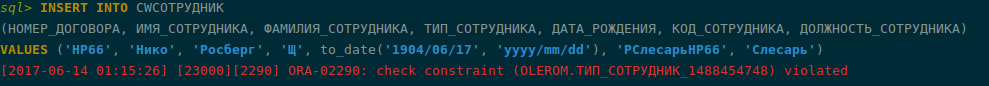
\includegraphics[width=17cm]{./screenshots/constraints/employee1.png}

    \item Должность\_сотрудника IN ('Сборщик', 'Токарь', 'Слесарь', 'Сварщик', 'Технолог', 'Техник', 'Инженер').
    Должности сотурдника на предприятии.

    \item Тип\_сотрудника || Должность\_сотрудника || Номер\_договора = Код\_сотрудника.
    Проверка соответствия кода сотрудника.

    \item  SUBSTR(Код\_сотрудника, 1, 1) = 'И'.
    Так мы не сможем добавит сотрудника и в ИТП, и в рабочих.

    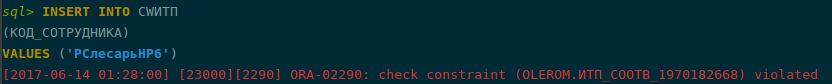
\includegraphics[width=17cm]{./screenshots/constraints/itp.png}

    \item SUBSTR(Код\_сотрудника, 1, 1) = 'Р'.
    Так мы не сможем добавит сотрудника и в ИТП, и в рабочих.

    \item Номер\_бригады >= 1.
    Чтобы номер бригады был положительным.

    \item Специализация\_сборщика IN ('двигатель', 'подвеска', 'кузов').
    То, в чем специализируется сборщик.

    \item SUBSTR(Код\_сотрудника, 2, 7) = 'Сборщик'.
    Так мы не сможем записать сразу в несколько категорий одного рабочего.
    Дальше аналогично для: токаря, слесаря, сварщика.

    \item Разряд\_токаря BETWEEN 1 AND 7.
    Возможные разряды токаря.

    \item Разряд\_слесаря BETWEEN 1 AND 6.
    Возможные разряды слесаря.

    \item Специализвация\_сварщика IN ('подвеска', 'рама').
    В сварке чего специализируется сварщик.

    \item SUBSTR(Код\_сотрудника, 2, 7) = 'Инженер'.
    Так мы не сможем записать сразу в несколько категорий одного представителя ИТП.
    Дальше аналогично для: техников и технологов.

    \item Специализация\_инженера IN ('проектирование', 'прототипирование').
    Специализация\_техника IN ('схемы', 'чертежи').
    Специализация\_технолога IN ('исследования', 'практика').
    В чем хороши конкретные преставители ИТП.

    \item Ответственность || Код\_сотрудника = Код\_ответств.
    Проверка соответствия кода ответсвенного.

    \item Ответственность IN ('Участок', 'Цех', 'Мастер').
    То, за что могут отвечать руководители.

    \item SUBSTR(Мастер, 1, 6) = 'Мастер'.
    Проверка на то, что в бригаде будет именно мастер, а не ркуоводитель цеха или участка.
    Так мы не сможем записать представителя ИТП в какую-нибудь другую ответсвенную позицию (начальник участка или цеха).

    \item (SUBSTR(Номер\_цеха, 1, 1) = 'П' OR SUBSTR(Номер\_цеха, 1, 1) = 'В') AND LENGTH(Номер\_цеха) = 4.
    Так мы можем записать префиксы П или В для цеха.
    П - производственный.
    В - вспомогательный.
    И будет невозможно записать цех и в вспомогательный, и в производственный. А в каждом подтипе есть проерка на соответсвие этому префиксу.

    \item SUBSTR(Начальник\_цеха, 1, 3) = 'Цех'.
    Только начальник цеха может быть начальником цеха.

    Попробуем записать мастера как отвественного за цех (начальник цеха), будет соответсвующая ошибка:

    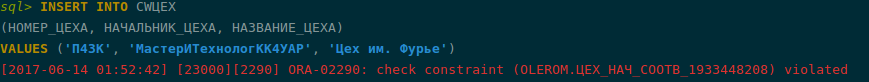
\includegraphics[width=17cm]{./screenshots/constraints/manufactory.png}

    \item SUBSTR(Код\_участка, 1, 4) = SUBSTR(Категорский\_цех, 1, 4).
    Проверяем соответствие цеха категории и цеха участка. Так данные будут согласованы.

    \item Вместимость >= 0.
    Вместимость автобуса должна быть положительным числов.

    \item SUBSTR(Код\_вида, 1, 8) = 'Автобусы'.
    Так мы не сможем записать сразу в несколько категорий.
    Аналогичная проверка для мотоциклов и грузовых автомобилей (также положительные числа для харрактеристик: например, грузоподъемность).

    \item Этап\_жизненного\_цикла IN ('Сборка', 'Передача дилеру', 'Гарантийный ремонт', 'Тестирование').
    Возможные этапы жизненного цикла.

    \item Начало < Конец.
    Окончание не может закончиться раньше, чем начало этапа цикла.

\end{itemize}

\section {Отчёт по замечаниям ERwin Data Model Validator}

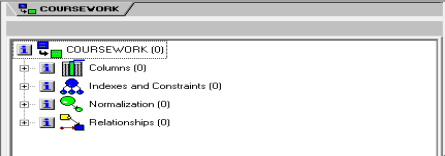
\includegraphics[width=17cm]{./screenshots/validator/validator.png}

Ошибок нет.

\section{Реализация запросов к базе данных}

\begin{enumerate}

    \item Перечень видов изделий по категории, собираемой указанным цехом.
    В последней строке вывести общее число собираемых видов изделий.

    Если вводят только цех через подстановочную переменную:

    \lstinputlisting[language=SQL]{../sources/queries/task1a.sql}

    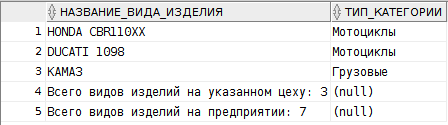
\includegraphics[width=16cm]{./screenshots/results/result1a.png}

    Если вводят цех и категорию через подстановочную переменную:

    \lstinputlisting[language=SQL]{../sources/queries/task1b.sql}

    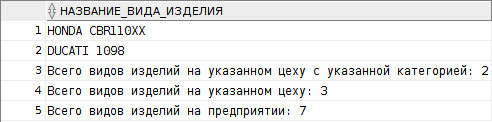
\includegraphics[width=16cm]{./screenshots/results/result1b.png}

    \item Количество экземпляров изделий каждого вида каждой категории, собранных предприятием за определенный отрезок времени.
    В последней строке вывести общее число собранных изделий.

    Если считать, что изделие собрано за отрезок времени: начало сборки больше начала отрезка и конец сборки меньше конца отрезка.

    \lstinputlisting[language=SQL]{../sources/queries/task2a.sql}

    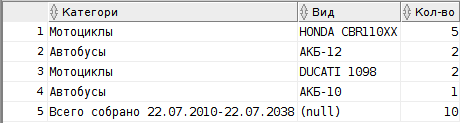
\includegraphics[width=16cm]{./screenshots/results/result2a.png}

    Если считать, что изделие собрано за отрезок времени: конца сборки больше начала отрезка и конец сборки меньше конца отрезка.

    \lstinputlisting[language=SQL]{../sources/queries/task2b.sql}

    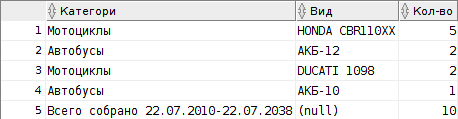
\includegraphics[width=16cm]{./screenshots/results/result2b.png}

    \item Данные о кадровом составе (ФИО, должность) по указанным категориям инженерно-технического персонала и рабочих;

    \lstinputlisting[language=SQL]{../sources/queries/task3.sql}

    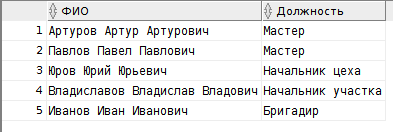
\includegraphics[width=16cm]{./screenshots/results/result3.png}

    \item Число и перечень участков предприятия и их начальников (с указанием цехов).

    \lstinputlisting[language=SQL]{../sources/queries/task4.sql}

    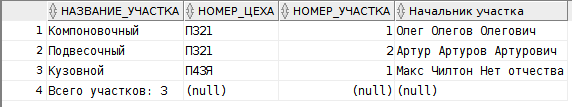
\includegraphics[width=16cm]{./screenshots/results/result4.png}

    \item Перечень работ, которые проходит указанный вид изделия.

    \lstinputlisting[language=SQL]{../sources/queries/task5.sql}

    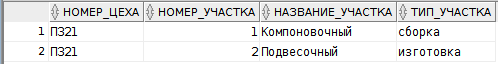
\includegraphics[width=16cm]{./screenshots/results/result5.png}

    \item Состав бригад, работающих на указанном участке указанного цеха: ФИО рабочего, номер бригады, номер участка, номер цеха. Отсортировать по номеру бригады.

    \lstinputlisting[language=SQL]{../sources/queries/task6.sql}

    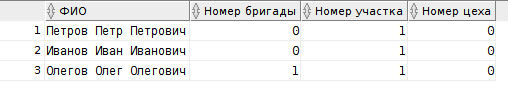
\includegraphics[width=16cm]{./screenshots/results/result6.png}

    \item Перечень мастеров (ФИО) указанного участка указанного цеха и номера бригад, работы которых они координируют.

    \lstinputlisting[language=SQL]{../sources/queries/task7.sql}

    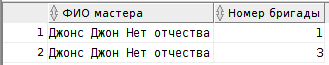
\includegraphics[width=16cm]{./screenshots/results/result7.png}

    \item Информация о цехах, в которых в настоящий момент собирается больше видов изделий, чем в среднем приходится на каждый производственный цех предприятия: номер цеха, название цеха, кол-во собираемых видов изделий, среднее количество видов изделий по цехам предприятия.

    \lstinputlisting[language=SQL]{../sources/queries/task8.sql}

    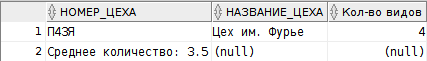
\includegraphics[width=16cm]{./screenshots/results/result8.png}

    \item Состав бригад, участвующих в сборке указанной категории изделия.

    \lstinputlisting[language=SQL]{../sources/queries/task9.sql}

    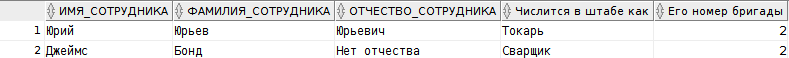
\includegraphics[width=16cm]{./screenshots/results/result9.png}

    \item ФИО и должности работников цеха, в котором собирается больше всего категорий изделий.

    \lstinputlisting[language=SQL]{../sources/queries/task10.sql}

    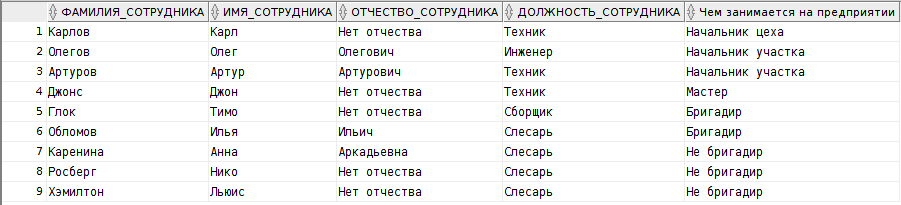
\includegraphics[width=16cm]{./screenshots/results/result10.png}

\end{enumerate}

\section{Создание представления}

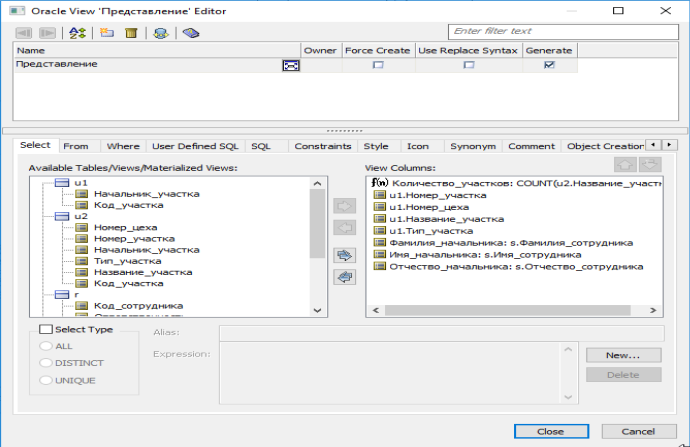
\includegraphics[width=16cm]{./screenshots/view/select_page.png}

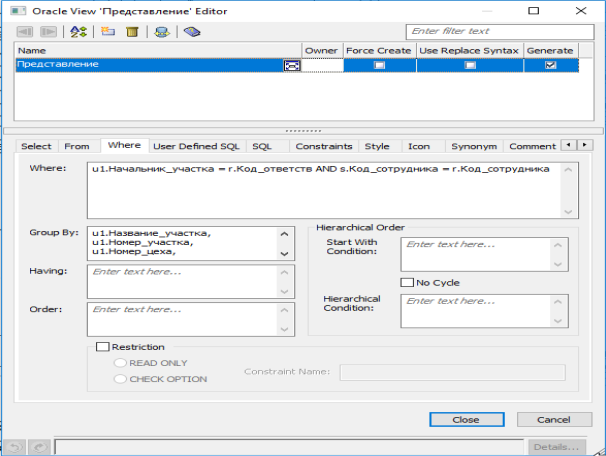
\includegraphics[width=16cm]{./screenshots/view/where_page.png}

Создал view представление запроса №4.
Однако с небольшим изменением, так как в 4 запросе использован UNION ALL, чтобы аккуратно добавить количество участков в конец таблицы.
А в представлении это же значение удалось вывести в первую колонку.

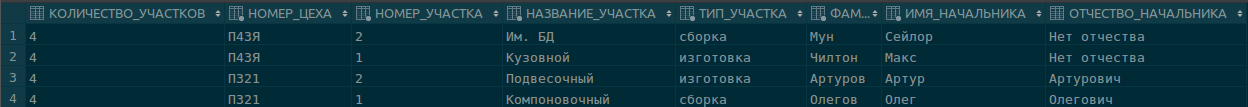
\includegraphics[width=16cm]{./screenshots/view/result.png}

\newpage

\section{Приложение 1}

    {\bf Физическая модель.}

    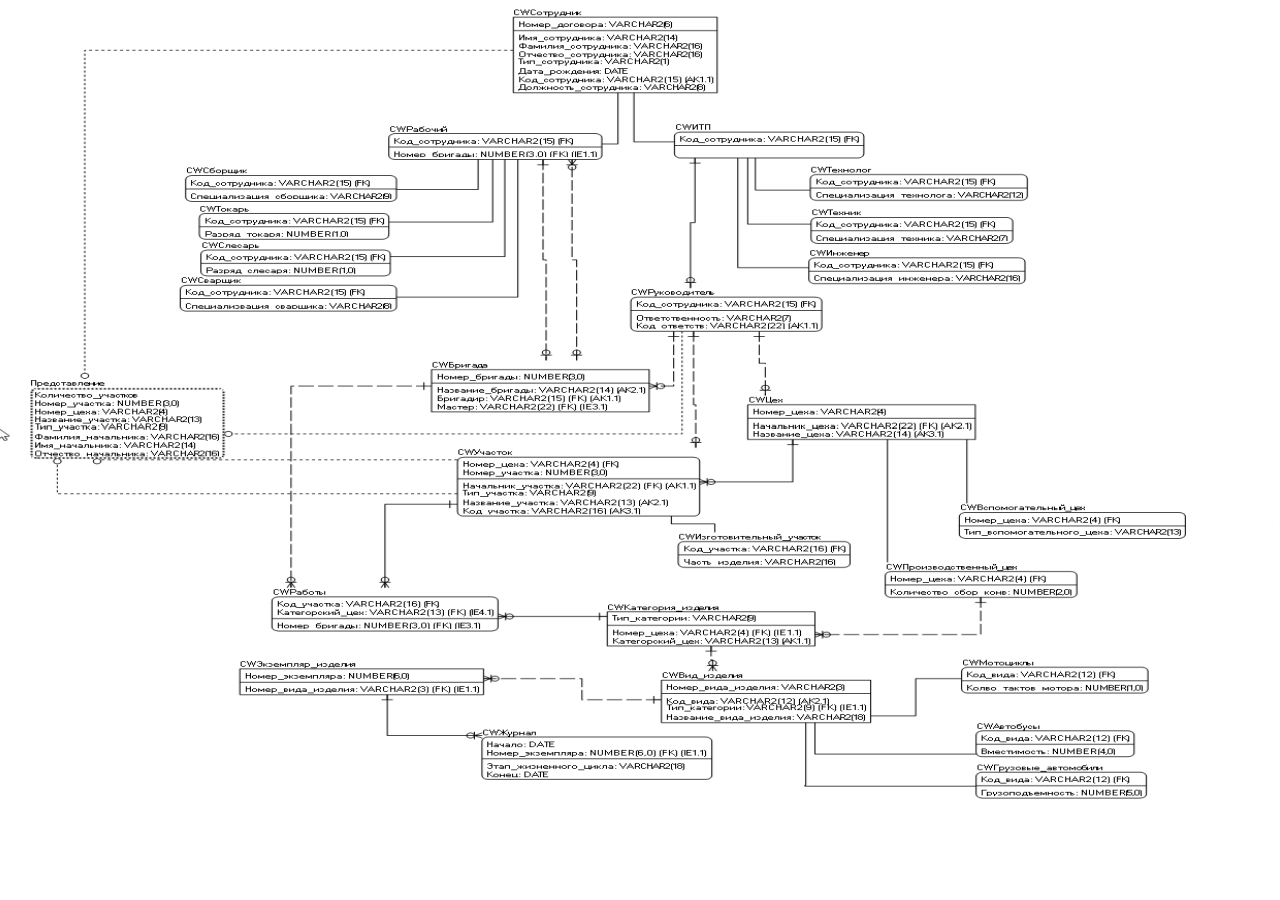
\includegraphics[width=16cm]{./screenshots/model/physical.png}

\newpage

\section{Приложение 2}

    {\bf Логическая модель.}

    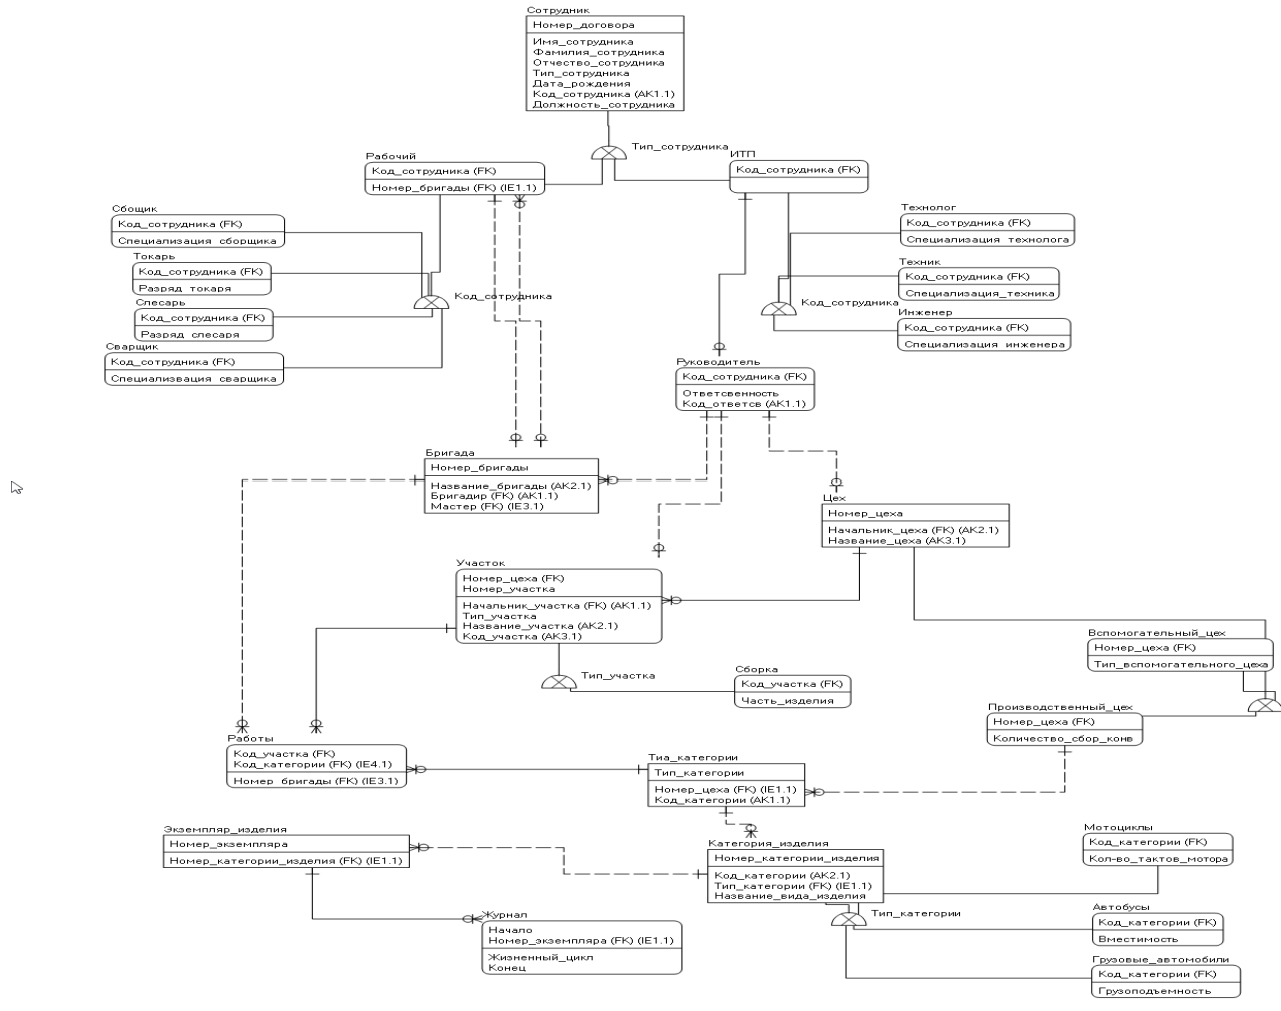
\includegraphics[width=16cm]{./screenshots/model/logical.png}

\newpage

\section{Приложение 3}

    {\bf Физическая модель после обратного проектирования.}

    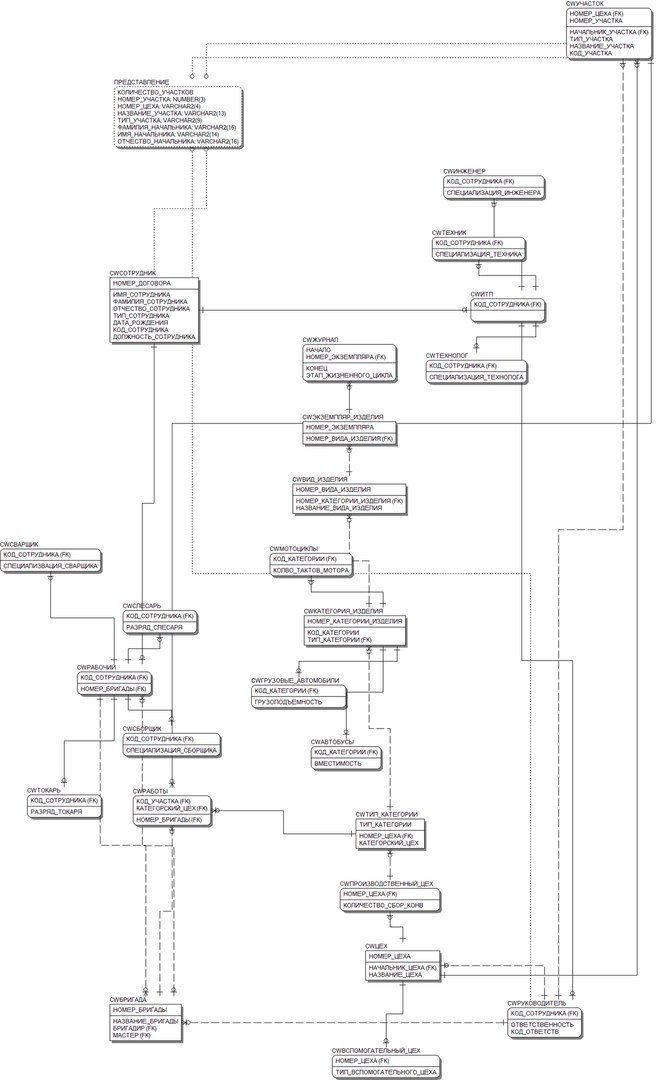
\includegraphics[width=16cm]{./screenshots/model/reverse.jpg}

\newpage

\section{Заключение}
В результате работы была спроектирована информационная система автомобилестроительного предприятия.
Была проведена нормализация разработанной модели до 5НФ.
Была проверена разработанная модель мредствами ERwin Data Model Validator r7, а также устранены все возможные замечания.
Проведено прямое и обратное проектирование.
Создано представление на основе 4 запроса.
Созданы 10 SQL-запросов и проверена их работоспособность.

Были закреплены теоретические и пркатические знания.

\section{Список использованных источников}

\begin{enumerate}

    \item Конспект лекций
    \item БАЗЫ ДАННЫХ. ПРАКТИКУМ. ЧАСТЬ 2. ORACLE SQL, О. Ю. Сабинин, Н. В. Андреева
    \item Материалы, доступные на dl.spbstu.ru

\end{enumerate}

\end{document}